\chapter{位运算}

计算机程序中的所有数据在内部都以比特，也就是数字 0 和 1 的形式存储。本章讨论整数的二进制表示，并通过示例说明如何使用位运算。事实证明，算法编程中有许多位运算的应用。

\section{二进制表示}

\index{bit representation}

在程序中，一个 $n$ 位整数在内部存储为由 $n$ 个比特组成的二进制数。例如，C++ 的 \texttt{int} 是 32 位类型，即每个 \texttt{int} 数由 32 个比特组成。

下面是 \texttt{int} 数 43 的二进制表示：
\[00000000000000000000000000101011\]
其中各位从右向左编号。要把二进制表示 $b_k\cdots b_2b_1b_0$ 转换为数值，可以使用公式
\[b_k 2^k + \ldots + b_2 2^2 + b_1 2^1 + b_0 2^0.\]
例如，
\[1 \cdot 2^5 + 1 \cdot 2^3 + 1 \cdot 2^1 + 1 \cdot 2^0 = 43.\]

数的二进制表示分为\key{有符号}和\key{无符号}两种。通常使用有符号表示，因此正数和负数都能表示。一个 $n$ 位有符号变量可保存 $-2^{n-1}$ 到 $2^{n-1}-1$ 之间的任意整数。例如，C++ 的 \texttt{int} 是有符号类型，可保存 $-2^{31}$ 到 $2^{31}-1$ 之间的任意整数。

有符号表示中的最高位是符号位（非负数为 0，负数为 1），其余 $n-1$ 位保存数值。实际使用\key{补码}表示，即先将一个数的所有位取反，再加一，就得到其相反数。

例如，\texttt{int} 数 $-43$ 的二进制表示为
\[11111111111111111111111111010101.\]

无符号表示只能用于非负数，但数值上界更大。一个 $n$ 位无符号变量可保存 $0$ 到 $2^n-1$ 之间的任意整数。例如，C++ 的 \texttt{unsigned int} 变量可保存 $0$ 到 $2^{32}-1$ 之间的任意整数。

两种表示之间存在联系：有符号数 $-x$ 等同于无符号数 $2^n-x$。例如，下列代码表明有符号数 $x=-43$ 等同于无符号数 $y=2^{32}-43$：
\begin{lstlisting}
int x = -43;
unsigned int y = x;
cout << x << "\n"; // -43
cout << y << "\n"; // 4294967253
\end{lstlisting}

若一个数超过二进制表示的上界，就会发生溢出。在有符号表示中，$2^{n-1}-1$ 之后的数是 $-2^{n-1}$；在无符号表示中，$2^n-1$ 之后的数是 0。例如，考虑下列代码：
\begin{lstlisting}
int x = 2147483647
cout << x << "\n"; // 2147483647
x++;
cout << x << "\n"; // -2147483648
\end{lstlisting}

初始时 $x=2^{31}-1$，这是 \texttt{int} 变量能保存的最大值，因此 $2^{31}-1$ 之后的数是 $-2^{31}$。


\section{位运算}

\newcommand\XOR{\mathbin{\char`\^}}

\subsubsection{按位与}

\index{and operation}

\key{按位与}运算 $x$ \& $y$ 产生一个数，只有 $x$ 和 $y$ 对应位都为 1 时，结果的该位才为 1。例如，$22$ \& $26$ = 18，因为

\begin{center}
\begin{tabular}{rrr}
& 10110 & (22)\\
\& & 11010 & (26) \\
\hline
 = & 10010 & (18) \\
\end{tabular}
\end{center}

利用按位与可以判断 $x$ 的奇偶性：若 $x$ 为偶数，则 $x$ \& $1$ = 0；若 $x$ 为奇数，则 $x$ \& $1$ = 1。更一般地，$x$ 能被 $2^k$ 整除，当且仅当 $x$ \& $(2^k-1)$ = 0。

\subsubsection{按位或}

\index{or operation}

\key{按位或}运算 $x$ | $y$ 产生一个数，只要 $x$ 和 $y$ 对应位中至少有一个为 1，结果的该位就为 1。例如，$22$ | $26$ = 30，因为

\begin{center}
\begin{tabular}{rrr}
& 10110 & (22)\\
| & 11010 & (26) \\
\hline
 = & 11110 & (30) \\
\end{tabular}
\end{center}

\subsubsection{按位异或}

\index{xor operation}

\key{按位异或}运算 $x$ $\XOR$ $y$ 产生一个数，只有 $x$ 和 $y$ 对应位中恰好一个为 1 时，结果的该位才为 1。例如，$22$ $\XOR$ $26$ = 12，因为

\begin{center}
\begin{tabular}{rrr}
& 10110 & (22)\\
$\XOR$ & 11010 & (26) \\
\hline
 = & 01100 & (12) \\
\end{tabular}
\end{center}

\subsubsection{按位取反}

\index{not operation}

\key{按位取反}运算 \textasciitilde$x$ 将 $x$ 的所有位翻转。恒有 \textasciitilde$x=-x-1$，例如 \textasciitilde$29=-30$。

取反运算在位层面的结果取决于二进制表示的长度，因为它会翻转所有位。例如，若使用 32 位 \texttt{int}，结果如下：

\begin{center}
\begin{tabular}{rrrr}
$x$ & = & 29 &   00000000000000000000000000011101 \\
\textasciitilde$x$ & = & $-30$ & 11111111111111111111111111100010 \\
\end{tabular}
\end{center}

\subsubsection{位移}

\index{bit shift}

左移 $x<<k$ 在数的末尾补上 $k$ 个零，右移 $x>>k$ 删除末尾 $k$ 位。例如，$14<<2=56$，因为 14 和 56 分别对应 1110 和 111000。同理，$49>>3=6$，因为 49 和 6 分别对应 110001 和 110。

注意，$x<<k$ 等价于将 $x$ 乘以 $2^k$，$x>>k$ 等价于将 $x$ 除以 $2^k$ 后向下取整。

\subsubsection{应用}

形如 $1<<k$ 的数只有第 $k$ 位为 1，其余位均为 0，因此可用它访问单个位。具体而言，一个数的第 $k$ 位为 1，当且仅当 $x$ \& $(1<<k)$ 非零。下列代码输出 \texttt{int} 数 $x$ 的二进制表示：

\begin{lstlisting}
for (int i = 31; i >= 0; i--) {
    if (x&(1<<i)) cout << "1";
    else cout << "0";
}
\end{lstlisting}

利用类似思想也可以修改单个位。例如，$x$ | $(1<<k)$ 将 $x$ 的第 $k$ 位置为 1；$x$ \& \textasciitilde $(1<<k)$ 将第 $k$ 位置为 0；$x$ $\XOR$ $(1<<k)$ 翻转第 $k$ 位。

表达式 $x$ \& $(x-1)$ 将 $x$ 最低的 1 位清零；$x$ \& $-x$ 将除最低 1 位外的所有 1 位清零；$x$ | $(x-1)$ 翻转最低 1 位之后的所有位。还要注意，正数 $x$ 是 2 的幂，当且仅当 $x$ \& $(x-1)=0$。

\subsubsection*{其他函数}

g++ 编译器提供下列位计数函数：

\begin{itemize}
\item
$\texttt{\_\_builtin\_clz}(x)$:
数的开头连续零的数量
\item
$\texttt{\_\_builtin\_ctz}(x)$:
数的末尾连续零的数量
\item
$\texttt{\_\_builtin\_popcount}(x)$:
数中 1 的数量
\item
$\texttt{\_\_builtin\_parity}(x)$:
数中 1 的数量的奇偶性
\end{itemize}
\begin{samepage}

这些函数可按如下方式使用：
\begin{lstlisting}
int x = 5328; // 00000000000000000001010011010000
cout << __builtin_clz(x) << "\n"; // 19
cout << __builtin_ctz(x) << "\n"; // 4
cout << __builtin_popcount(x) << "\n"; // 5
cout << __builtin_parity(x) << "\n"; // 1
\end{lstlisting}
\end{samepage}

上述函数只支持 \texttt{int}，但也有以 \texttt{ll} 为后缀、支持 \texttt{long long} 的版本。

\section{集合的表示}

集合 $\{0,1,2,\ldots,n-1\}$ 的每个子集都可表示为一个 $n$ 位整数，其中为 1 的位指出哪些元素属于该子集。这是一种高效的集合表示方式，因为每个元素只占一个比特，并且集合运算可以实现为位运算。

例如，由于 \texttt{int} 是 32 位类型，一个 \texttt{int} 数可以表示集合 $\{0,1,2,\ldots,31\}$ 的任意子集。集合 $\{1,3,4,8\}$ 的二进制表示为
\[00000000000000000000000100011010,\]
对应数值 $2^8+2^4+2^3+2^1=282$。

\subsubsection{集合实现}

下列代码声明一个 \texttt{int} 变量 $x$，用于保存 $\{0,1,2,\ldots,31\}$ 的子集。随后，代码把元素 1、3、4 和 8 加入集合，并输出集合大小。
\begin{lstlisting}
int x = 0;
x |= (1<<1);
x |= (1<<3);
x |= (1<<4);
x |= (1<<8);
cout << __builtin_popcount(x) << "\n"; // 4
\end{lstlisting}
下列代码输出属于该集合的所有元素：
\begin{lstlisting}
for (int i = 0; i < 32; i++) {
    if (x&(1<<i)) cout << i << " ";
}
// output: 1 3 4 8
\end{lstlisting}

\subsubsection{集合运算}

集合运算可以实现为如下位运算：

\begin{center}
\begin{tabular}{lll}
& 集合写法 & 位运算写法 \\
\hline
交集 & $a \cap b$ & $a$ \& $b$ \\
并集 & $a \cup b$ & $a$ | $b$ \\
补集 & $\bar a$ & \textasciitilde$a$ \\
差集 & $a \setminus b$ & $a$ \& (\textasciitilde$b$) \\
\end{tabular}
\end{center}

例如，下列代码先构造集合 $x=\{1,3,4,8\}$ 与 $y=\{3,6,8,9\}$，再构造集合 $z=x\cup y=\{1,3,4,6,8,9\}$：

\begin{lstlisting}
int x = (1<<1)|(1<<3)|(1<<4)|(1<<8);
int y = (1<<3)|(1<<6)|(1<<8)|(1<<9);
int z = x|y;
cout << __builtin_popcount(z) << "\n"; // 6
\end{lstlisting}

\subsubsection{遍历子集}

下列代码遍历 $\{0,1,\ldots,n-1\}$ 的所有子集：

\begin{lstlisting}
for (int b = 0; b < (1<<n); b++) {
    // process subset b
}
\end{lstlisting}
下列代码遍历恰含 $k$ 个元素的子集：
\begin{lstlisting}
for (int b = 0; b < (1<<n); b++) {
    if (__builtin_popcount(b) == k) {
        // process subset b
    }
}
\end{lstlisting}
下列代码遍历集合 $x$ 的所有子集：
\begin{lstlisting}
int b = 0;
do {
    // process subset b
} while (b=(b-x)&x);
\end{lstlisting}

\section{位运算优化}

许多算法都可以用位运算优化。这类优化不会改变算法的时间复杂度，却可能显著影响代码的实际运行时间。本节讨论几个这样的例子。

\subsubsection{Hamming 距离}

\index{Hamming distance}
两个等长字符串 $a$ 和 $b$ 之间的\key{Hamming 距离} $\texttt{hamming}(a,b)$ 是二者字符不同的位置数。例如，
\[\texttt{hamming}(01101,11001)=2.\]

考虑如下问题：给定 $n$ 个长度均为 $k$ 的比特串，计算列表中两个字符串之间的最小 Hamming 距离。例如，$[00111,01101,11110]$ 的答案为 2，因为
\begin{itemize}[noitemsep]
\item $\texttt{hamming}(00111,01101)=2$,
\item $\texttt{hamming}(00111,11110)=3$, and
\item $\texttt{hamming}(01101,11110)=3$.
\end{itemize}

直接解法是遍历所有字符串对并计算 Hamming 距离，得到 $O(n^2k)$ 时间算法。下列函数可用于计算距离：
\begin{lstlisting}
int hamming(string a, string b) {
    int d = 0;
    for (int i = 0; i < k; i++) {
        if (a[i] != b[i]) d++;
    }
    return d;
}
\end{lstlisting}

若 $k$ 较小，可以把比特串存为整数，并用位运算计算 Hamming 距离来优化代码。特别地，若 $k\le32$，可以直接把字符串存为 \texttt{int}，并用下列函数计算距离：
\begin{lstlisting}
int hamming(int a, int b) {
    return __builtin_popcount(a^b);
}
\end{lstlisting}
上述函数中，异或运算构造出一个在 $a$ 与 $b$ 不同位置为 1 的比特串，再用 \texttt{\_\_builtin\_popcount} 统计 1 的数量。

为比较两种实现，我们生成了 10000 个长度为 30 的随机比特串。第一种方法耗时 13.5 秒，位运算优化后只需 0.5 秒。因此，优化后的代码几乎比原代码快 30 倍。

\subsubsection{子网格计数}

再考虑如下问题：给定一个 $n\times n$ 网格，每个方格为黑色（1）或白色（0），计算四个角均为黑色的子网格数量。例如，网格
\begin{center}
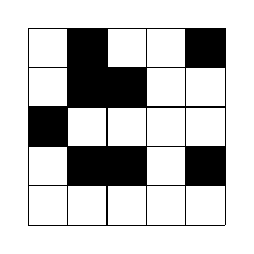
\begin{tikzpicture}[scale=0.5]
\fill[black] (1,1) rectangle (2,2);
\fill[black] (1,4) rectangle (2,5);
\fill[black] (4,1) rectangle (5,2);
\fill[black] (4,4) rectangle (5,5);
\fill[black] (1,3) rectangle (2,4);
\fill[black] (2,3) rectangle (3,4);
\fill[black] (2,1) rectangle (3,2);
\fill[black] (0,2) rectangle (1,3);
\draw (0,0) grid (5,5);
\end{tikzpicture}
\end{center}
包含两个这样的子网格：
\begin{center}
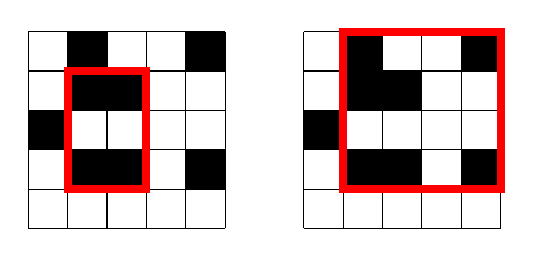
\begin{tikzpicture}[scale=0.5]
\fill[black] (1,1) rectangle (2,2);
\fill[black] (1,4) rectangle (2,5);
\fill[black] (4,1) rectangle (5,2);
\fill[black] (4,4) rectangle (5,5);
\fill[black] (1,3) rectangle (2,4);
\fill[black] (2,3) rectangle (3,4);
\fill[black] (2,1) rectangle (3,2);
\fill[black] (0,2) rectangle (1,3);
\draw (0,0) grid (5,5);

\fill[black] (7+1,1) rectangle (7+2,2);
\fill[black] (7+1,4) rectangle (7+2,5);
\fill[black] (7+4,1) rectangle (7+5,2);
\fill[black] (7+4,4) rectangle (7+5,5);
\fill[black] (7+1,3) rectangle (7+2,4);
\fill[black] (7+2,3) rectangle (7+3,4);
\fill[black] (7+2,1) rectangle (7+3,2);
\fill[black] (7+0,2) rectangle (7+1,3);
\draw (7+0,0) grid (7+5,5);

\draw[color=red,line width=1mm] (1,1) rectangle (3,4);
\draw[color=red,line width=1mm] (7+1,1) rectangle (7+5,5);
\end{tikzpicture}
\end{center}

有一种 $O(n^3)$ 时间算法：遍历 $O(n^2)$ 对行，对每一对 $(a,b)$，在 $O(n)$ 时间内计算有多少列在这两行中都含黑色方格。下列代码假设 $\texttt{color}[y][x]$ 表示第 $y$ 行第 $x$ 列的颜色：
\begin{lstlisting}
int count = 0;
for (int i = 0; i < n; i++) {
    if (color[a][i] == 1 && color[b][i] == 1) count++;
}
\end{lstlisting}
这些列会形成 $\texttt{count}(\texttt{count}-1)/2$ 个四角为黑色的子网格，因为可任选其中两列组成一个子网格。

为优化该算法，把网格按列分块，每块由连续的 $N$ 列组成。随后将每一行存为一列 $N$ 位整数，用以描述方格颜色。这样便可用位运算同时处理 $N$ 列。下列代码中，$\texttt{color}[y][k]$ 以比特形式表示一块 $N$ 个颜色：
\begin{lstlisting}
int count = 0;
for (int i = 0; i <= n/N; i++) {
    count += __builtin_popcount(color[a][i]&color[b][i]);
}
\end{lstlisting}
所得算法的时间复杂度为 $O(n^3/N)$。

我们生成了一个 $2500\times2500$ 的随机网格，并比较原始实现与位运算优化实现。原代码耗时 $29.6$ 秒，而优化版本在 $N=32$（\texttt{int}）时只需 $3.1$ 秒，在 $N=64$（\texttt{long long}）时只需 $1.7$ 秒。

\section{动态规划}

对于状态中包含元素子集的动态规划算法，位运算提供了一种高效方便的实现方式，因为这类状态可以存为整数。下面讨论结合位运算与动态规划的例子。

\subsubsection{最优选择}

第一个例子如下：已知 $k$ 种商品在 $n$ 天中的价格，希望每种商品恰好购买一次，但每天至多购买一种商品。最小总价是多少？例如，考虑下列情形（$k=3$，$n=8$）：
\begin{center}
\begin{tikzpicture}[scale=.65]
    \draw (0, 0) grid (8,3);
    \node at (-2.5,2.5) {商品 0};
    \node at (-2.5,1.5) {商品 1};
    \node at (-2.5,0.5) {商品 2};

    \foreach \x in {0,...,7}
        {\node at (\x+0.5,3.5) {\x};}
    \foreach \x/\v in {0/6,1/9,2/5,3/2,4/8,5/9,6/1,7/6}
        {\node at (\x+0.5,2.5) {\v};}
    \foreach \x/\v in {0/8,1/2,2/6,3/2,4/7,5/5,6/7,7/2}
        {\node at (\x+0.5,1.5) {\v};}
    \foreach \x/\v in {0/5,1/3,2/9,3/7,4/3,5/5,6/1,7/4}
        {\node at (\x+0.5,0.5) {\v};}
\end{tikzpicture}
\end{center}
此时最小总价为 $5$：
\begin{center}
\begin{tikzpicture}[scale=.65]
    \fill [color=lightgray] (1, 1) rectangle (2, 2);
    \fill [color=lightgray] (3, 2) rectangle (4, 3);
    \fill [color=lightgray] (6, 0) rectangle (7, 1);
    \draw (0, 0) grid (8,3);
    \node at (-2.5,2.5) {商品 0};
    \node at (-2.5,1.5) {商品 1};
    \node at (-2.5,0.5) {商品 2};

    \foreach \x in {0,...,7}
        {\node at (\x+0.5,3.5) {\x};}
    \foreach \x/\v in {0/6,1/9,2/5,3/2,4/8,5/9,6/1,7/6}
        {\node at (\x+0.5,2.5) {\v};}
    \foreach \x/\v in {0/8,1/2,2/6,3/2,4/7,5/5,6/7,7/2}
        {\node at (\x+0.5,1.5) {\v};}
    \foreach \x/\v in {0/5,1/3,2/9,3/7,4/3,5/5,6/1,7/4}
        {\node at (\x+0.5,0.5) {\v};}
\end{tikzpicture}
\end{center}

令 $\texttt{price}[x][d]$ 表示商品 $x$ 在第 $d$ 天的价格。例如，上述情形中 $\texttt{price}[2][3]=7$。再令 $\texttt{total}(S,d)$ 表示截至第 $d$ 天购买商品子集 $S$ 的最小总价，则问题答案为 $\texttt{total}(\{0\ldots k-1\},n-1)$。

首先，$\texttt{total}(\emptyset,d)=0$，因为购买空集无需花费；且 $\texttt{total}(\{x\},0)=\texttt{price}[x][0]$，因为第一天购买一种商品只有一种方式。随后使用递推式：
\begin{equation*}
\begin{split}
\texttt{total}(S,d) = \min( & \texttt{total}(S,d-1), \\
& \min_{x \in S} (\texttt{total}(S \setminus x,d-1)+\texttt{price}[x][d]))
\end{split}
\end{equation*}
这表示第 $d$ 天要么不买任何商品，要么购买属于 $S$ 的商品 $x$。后一种情形中，从 $S$ 删除 $x$，并把 $x$ 的价格加入总价。

下一步用动态规划计算函数值。声明数组保存函数值：
\begin{lstlisting}
int total[1<<K][N];
\end{lstlisting}
其中 $K$ 和 $N$ 是足够大的常量。数组第一维对应子集的二进制表示。

首先，按如下方式处理 $d=0$ 的情形：
\begin{lstlisting}
for (int x = 0; x < k; x++) {
    total[1<<x][0] = price[x][0];
}
\end{lstlisting}
随后，递推式转化为下列代码：
\begin{lstlisting}
for (int d = 1; d < n; d++) {
    for (int s = 0; s < (1<<k); s++) {
        total[s][d] = total[s][d-1];
        for (int x = 0; x < k; x++) {
            if (s&(1<<x)) {
                total[s][d] = min(total[s][d],
                                    total[s^(1<<x)][d-1]+price[x][d]);
            }
        }
    }
}
\end{lstlisting}
算法的时间复杂度为 $O(n2^kk)$。

\subsubsection{从排列到子集}

利用动态规划，常可把对排列的遍历转化为对子集的遍历\footnote{该技术由 M. Held 和 R. M. Karp 于 1962 年提出 \cite{hel62}。}。这样做的好处是，排列数 $n!$ 远大于子集数 $2^n$。例如，当 $n=20$ 时，$n!\approx2.4\cdot10^{18}$，而 $2^n\approx10^6$。因此，对某些 $n$，可以高效遍历子集，却无法遍历排列。

例如，考虑如下问题：一部电梯的最大载重为 $x$，有 $n$ 个体重已知的人想从底层到顶层。若按最优顺序进入电梯，最少需要运行多少趟？

例如，设 $x=10$、$n=5$，各人体重如下：
\begin{center}
\begin{tabular}{ll}
人员 & 体重 \\
\hline
0 & 2 \\
1 & 3 \\
2 & 3 \\
3 & 5 \\
4 & 6 \\
\end{tabular}
\end{center}
此时最少需要 2 趟。一种最优顺序为 $\{0,2,3,1,4\}$，将人员分为两趟：先运送 $\{0,2,3\}$（总重 10），再运送 $\{1,4\}$（总重 9）。

测试 $n$ 个人的所有排列，可以轻松在 $O(n!n)$ 时间内解决问题。不过，使用动态规划可以得到更高效的 $O(2^nn)$ 时间算法。其思想是为每个人员子集计算两个值：所需的最少趟数，以及最后一趟的最小总重。

令 $\texttt{weight}[p]$ 表示人员 $p$ 的体重。定义两个函数：$\texttt{rides}(S)$ 是子集 $S$ 所需的最少趟数，$\texttt{last}(S)$ 是最后一趟的最小总重。例如，在上述情形中
\[ \texttt{rides}(\{1,3,4\})=2 \hspace{10pt} \textrm{且}
\hspace{10pt} \texttt{last}(\{1,3,4\})=5,\]
因为最优的两趟为 $\{1,4\}$ 和 $\{3\}$，第二趟总重为 5。最终目标当然是计算 $\texttt{rides}(\{0\ldots n-1\})$。

可以递归计算函数值，再应用动态规划。遍历属于 $S$ 的所有人员，最优地选择最后进入电梯的人 $p$。每种选择都会产生一个更小人员子集的子问题。若 $\texttt{last}(S\setminus p)+\texttt{weight}[p]\le x$，可以把 $p$ 加入最后一趟；否则必须另开一趟，起初只包含 $p$。

为实现动态规划，声明数组
\begin{lstlisting}
pair<int,int> best[1<<N];
\end{lstlisting}
为每个子集 $S$ 保存二元组 $(\texttt{rides}(S),\texttt{last}(S))$。空集的值如下：
\begin{lstlisting}
best[0] = {1,0};
\end{lstlisting}
随后按如下方式填充数组：

\begin{lstlisting}
for (int s = 1; s < (1<<n); s++) {
    // initial value: n+1 rides are needed
    best[s] = {n+1,0};
    for (int p = 0; p < n; p++) {
        if (s&(1<<p)) {
            auto option = best[s^(1<<p)];
            if (option.second+weight[p] <= x) {
                // add p to an existing ride
                option.second += weight[p];
            } else {
                // reserve a new ride for p
                option.first++;
                option.second = weight[p];
            }
            best[s] = min(best[s], option);
        }
    }
}
\end{lstlisting}
注意，上述循环保证对任意满足 $S_1\subset S_2$ 的两个子集 $S_1$ 和 $S_2$，总是先处理 $S_1$。因此，动态规划值按正确顺序计算。

\subsubsection{子集计数}

本章最后一个问题如下：令 $X=\{0\ldots n-1\}$，并为每个子集 $S\subset X$ 赋予整数 $\texttt{value}[S]$。需要对每个 $S$ 计算
\[\texttt{sum}(S) = \sum_{A \subset S} \texttt{value}[A],\]
即 $S$ 的所有子集的值之和。

例如，设 $n=3$，各值如下：
\begin{multicols}{2}
\begin{itemize}
\item $\texttt{value}[\emptyset] = 3$
\item $\texttt{value}[\{0\}] = 1$
\item $\texttt{value}[\{1\}] = 4$
\item $\texttt{value}[\{0,1\}] = 5$
\item $\texttt{value}[\{2\}] = 5$
\item $\texttt{value}[\{0,2\}] = 1$
\item $\texttt{value}[\{1,2\}] = 3$
\item $\texttt{value}[\{0,1,2\}] = 3$
\end{itemize}
\end{multicols}
此时，例如，
\begin{equation*}
\begin{split}
\texttt{sum}(\{0,2\}) &= \texttt{value}[\emptyset]+\texttt{value}[\{0\}]+\texttt{value}[\{2\}]+\texttt{value}[\{0,2\}] \\ 
                      &= 3 + 1 + 5 + 1 = 10.
\end{split}
\end{equation*}

由于共有 $2^n$ 个子集，一种解法是在 $O(2^{2n})$ 时间内遍历所有子集对。不过，使用动态规划可以在 $O(2^nn)$ 时间内解决问题。其思想是限制可以从 $S$ 中删除的元素，并研究相应的和。

令 $\texttt{partial}(S,k)$ 表示 $S$ 的所有满足“只能删除元素 $0\ldots k$”这一限制的子集的值之和。例如，
\[\texttt{partial}(\{0,2\},1)=\texttt{value}[\{2\}]+\texttt{value}[\{0,2\}],\]
因为只能删除元素 $0\ldots1$。可以用 \texttt{partial} 计算 \texttt{sum}，因为
\[\texttt{sum}(S) = \texttt{partial}(S,n-1).\]
函数的基本情形为
\[\texttt{partial}(S,-1)=\texttt{value}[S],\]
因为此时不能从 $S$ 中删除任何元素。一般情形使用下列递推式：
\begin{equation*}
    \texttt{partial}(S,k) = \begin{cases}
               \texttt{partial}(S,k-1) & k \notin S \\
               \texttt{partial}(S,k-1) + \texttt{partial}(S \setminus \{k\},k-1) & k \in S
           \end{cases}
\end{equation*}
这里关注元素 $k$。若 $k\in S$，有两种选择：在 $S$ 中保留 $k$，或从 $S$ 删除 $k$。

有一种特别巧妙的方式实现这些和的计算。声明数组
\begin{lstlisting}
int sum[1<<N];
\end{lstlisting}
保存每个子集的和。数组初始化如下：
\begin{lstlisting}
for (int s = 0; s < (1<<n); s++) {
    sum[s] = value[s];
}
\end{lstlisting}
随后按如下方式填充数组：
\begin{lstlisting}
for (int k = 0; k < n; k++) {
    for (int s = 0; s < (1<<n); s++) {
        if (s&(1<<k)) sum[s] += sum[s^(1<<k)];
    }
}
\end{lstlisting}
该代码把 $k=0\ldots n-1$ 时的 $\texttt{partial}(S,k)$ 依次计算到数组 \texttt{sum} 中。由于 $\texttt{partial}(S,k)$ 总是以 $\texttt{partial}(S,k-1)$ 为基础，可以复用数组 \texttt{sum}，从而得到非常高效的实现。
